\documentclass{beamer}
\usepackage[utf8]{inputenc}
\usetheme{Berlin}
\usepackage[spanish]{babel}
\usepackage{multirow}
%\usepackage{estilo-apuntes}
\usepackage[]{graphicx}
\usepackage{svg}

\theoremstyle{definition}

\newtheorem{teorema}{Teorema}
\newtheorem{defi}{Definición}
\newtheorem{prop}[teorema]{Proposición}
\newcommand{\Z}{\mathbb{Z}}
\newcommand{\C}{\mathbb{C}}
\newcommand{\D}{\mathbb{D}}
\providecommand{\gene}[1]{\langle{#1}\rangle}

\addtobeamertemplate{navigation symbols}{}{%
    \usebeamerfont{footline}%
    \usebeamercolor[fg]{footline}%
    \hspace{1em}%
    \insertframenumber/\inserttotalframenumber
}
\setbeamercolor{footline}{fg=black}
\setbeamerfont{footline}{series=\bfseries}

%-----------------------------------------------------------

\title{Modelo basado en árboles}
\author{Diego Pedrazo, Daniel García, Rafael González}
\institute{Universidad de Sevilla}
\date{}
 
\begin{document}
\frame{\titlepage}

\begin{frame}
\frametitle{Tabla de contenidos}
\tableofcontents
\end{frame}
%}

\section{Estratificación}

\begin{frame}
\begin{figure}[h!]
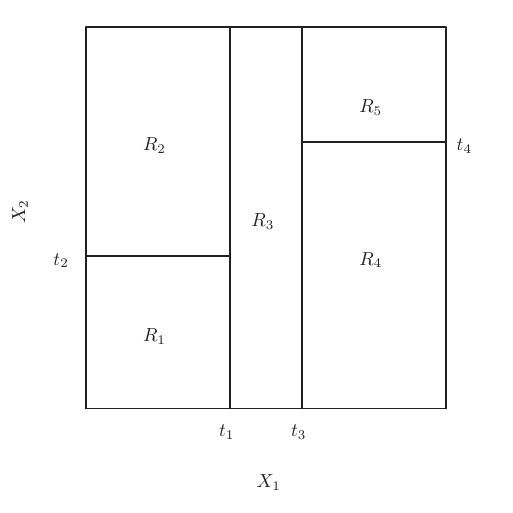
\includegraphics[scale=0.4]{regiones}
\end{figure}
\end{frame}

\begin{frame}
\begin{figure}[h!]
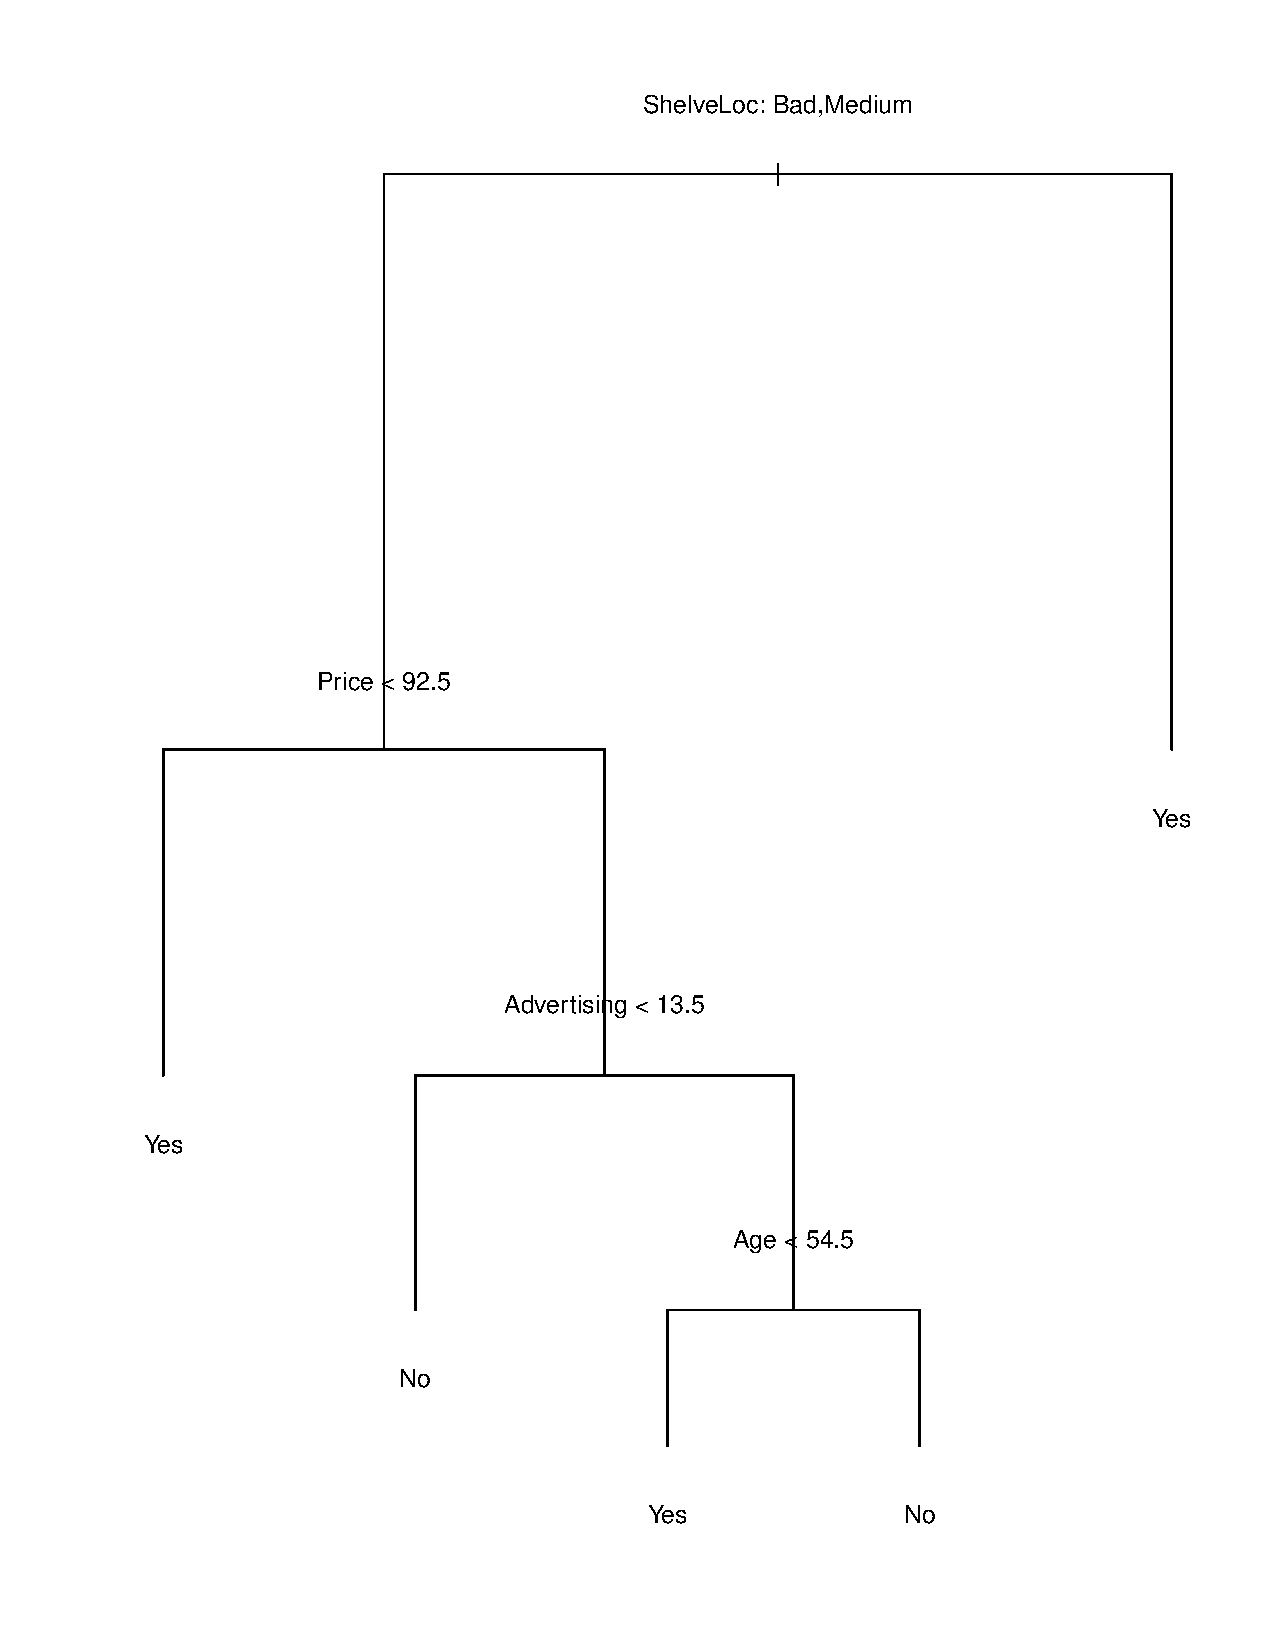
\includegraphics[scale=0.28]{grafo1}
\end{figure}
\end{frame}

\section{Recursive Binary Splitting}


\begin{frame}
\begin{center}
Suma de los residuios al cuadrado (RSS)
\end{center}
\[ \min \sum_{j=1}^J\sum_{i\in R_j}(y_i-\hat{y}_{R_j})^2 \]
\end{frame}


\begin{frame}
\begin{figure}[h!]
%\includesvg[scale=0.5]{dibujo}
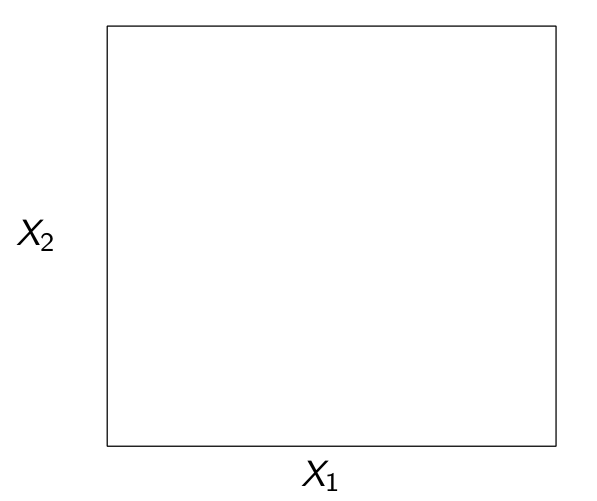
\includegraphics[scale=0.3]{svg-inkscape/dibujo.png}
\end{figure}
\end{frame}

\begin{frame}
\begin{figure}[h!]
%\includesvg[scale=0.5]{dibujo2}
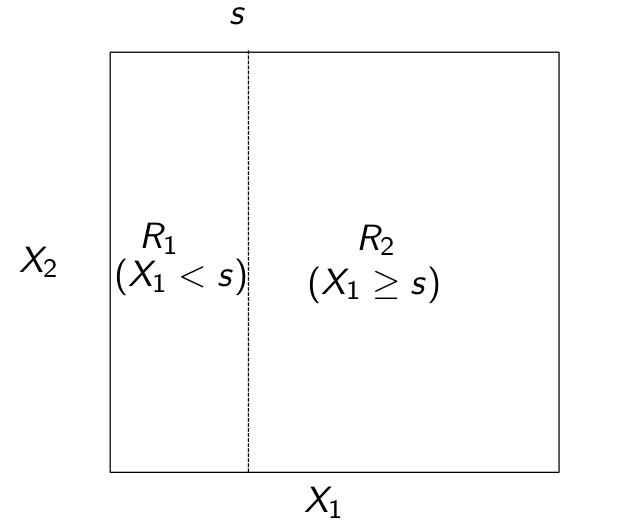
\includegraphics[scale=0.3]{svg-inkscape/dibujo2.png}
\end{figure}
\end{frame}

\begin{frame}
\[ \min \sum_{i\colon x_i \in R_1(j,s)} (y_i - \widehat{y}_{R_1})^2 + \sum_{i\colon x_i \in R_2(j,s)} (y_i - \widehat{y}_{R_2})^2 \]
\end{frame}

\begin{frame}
\begin{figure}[h!]
%\includesvg[scale=0.5]{dibujo3}
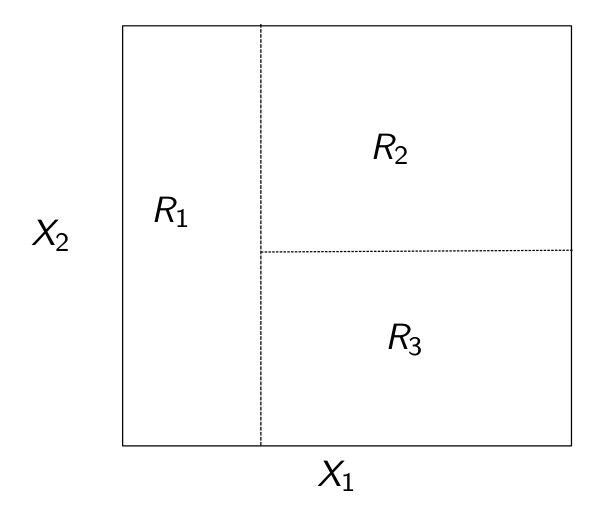
\includegraphics[scale=0.3]{svg-inkscape/dibujo3.png}
\end{figure}
\end{frame}


\begin{frame}
\begin{figure}[h!]
%includesvg[scale=0.5]{dibujo4}
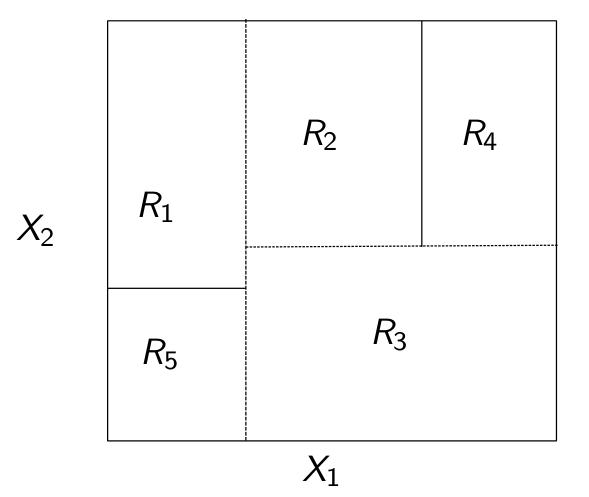
\includegraphics[scale=0.3]{svg-inkscape/dibujo4.png}
\end{figure}
\end{frame}

\section{Prunning}
\begin{frame}
\begin{figure}[h!]
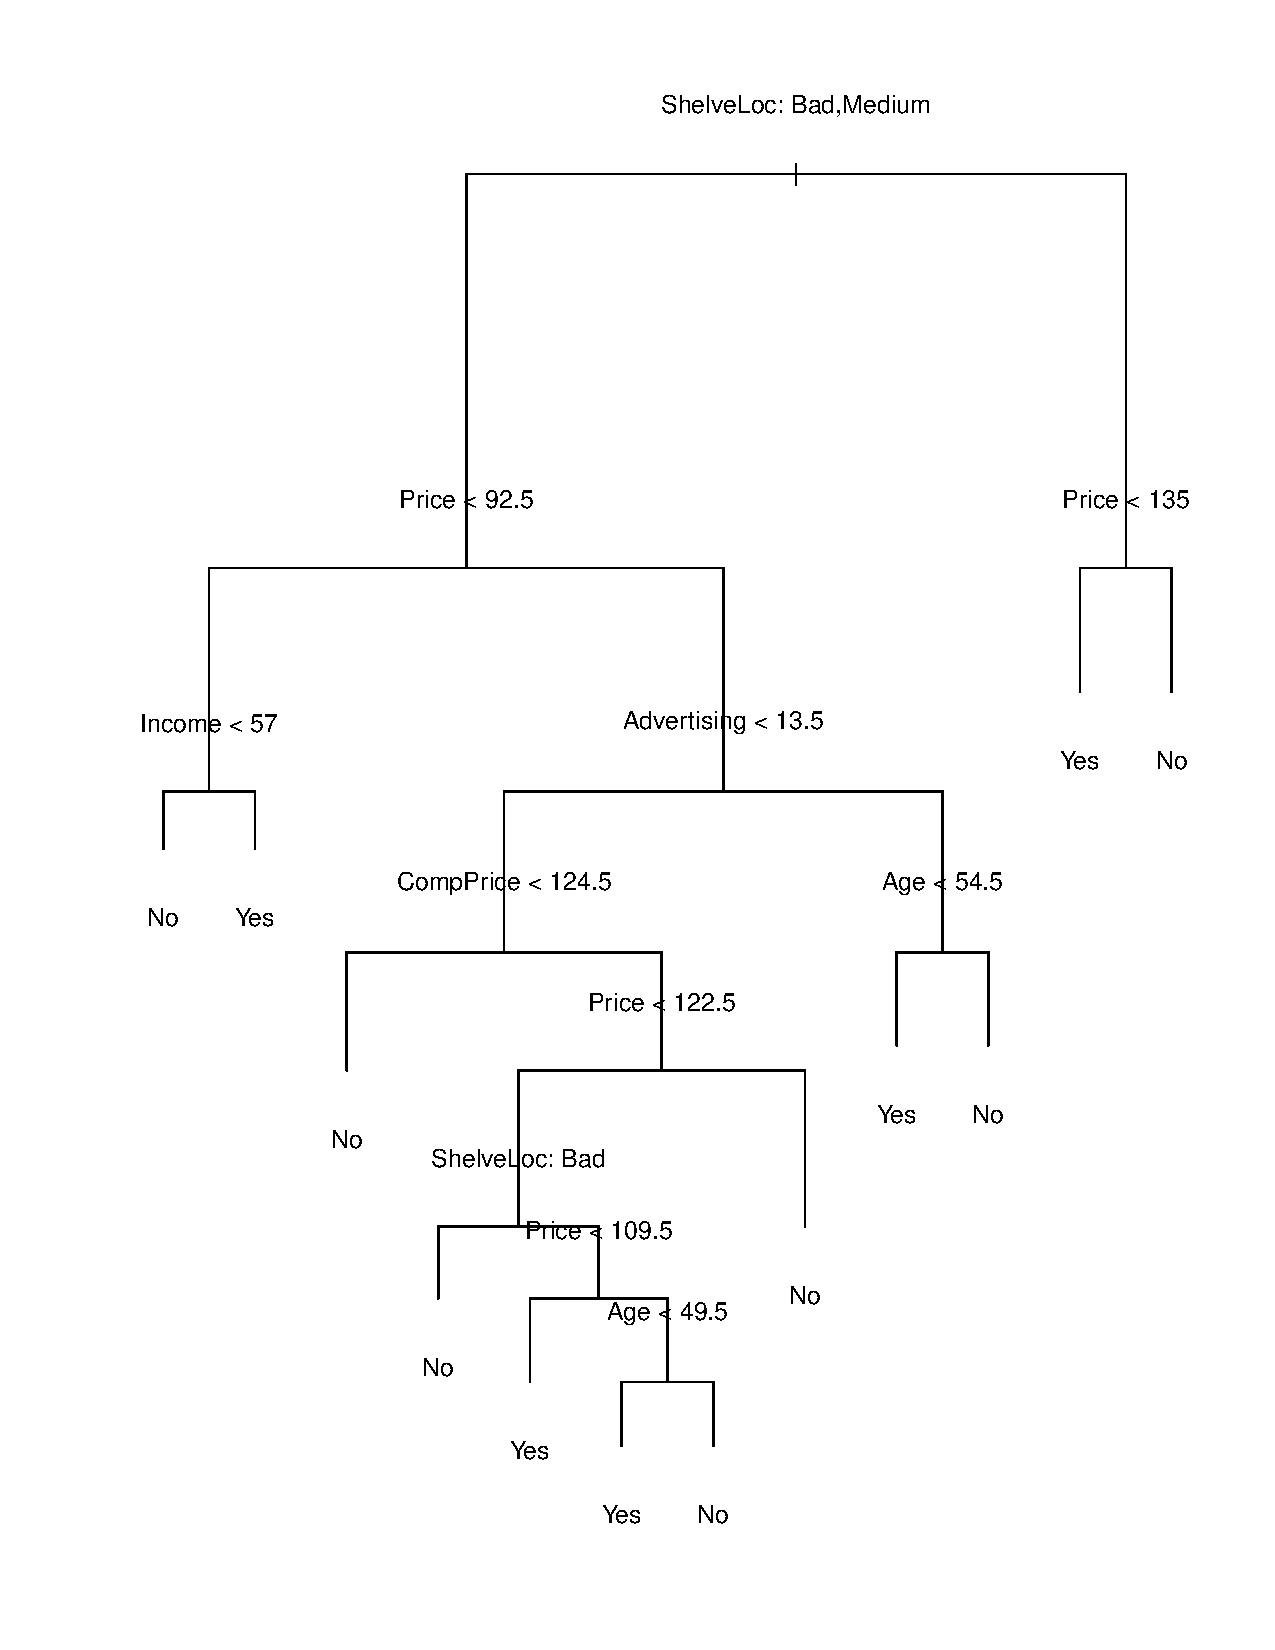
\includegraphics[scale=0.28]{arbolgrande}
\end{figure}
\end{frame}

\begin{frame}
\begin{enumerate}
	\item<1-> Crea un árbol grande $T_0$.
	\item<2-> Para cada valor $\alpha$, encuentra el subárbol $T$ que minimiza
	\[ \sum_{m=1}^{|T|} \sum_{i\colon x_I \in R_m} (y_i - \widehat{y}_{R_m})^2 + \alpha|T| \]
	\item<3-> Usamos $K$-fold cross-validation para elegir $\alpha$.
	\item<4-> Devuelve su correspondiente árbol.
\end{enumerate}
\end{frame}
\section{Clasificación}

\begin{frame}
\begin{gather*}
 E = 1 - \max(\hat{p}_{mk}) \\ 
 G = \sum_{k=1}^K \hat{p}_{mk}(1-\hat{p}_{mk})\\
  D = -\sum_{k=1}^K \hat{p}_{mk} \log \hat{p}_{mk}
\end{gather*}
\end{frame}

\section{Comparativa}
\begin{frame}
\begin{figure}[h!]
%\includesvg[scale=0.5]{dibujo3}
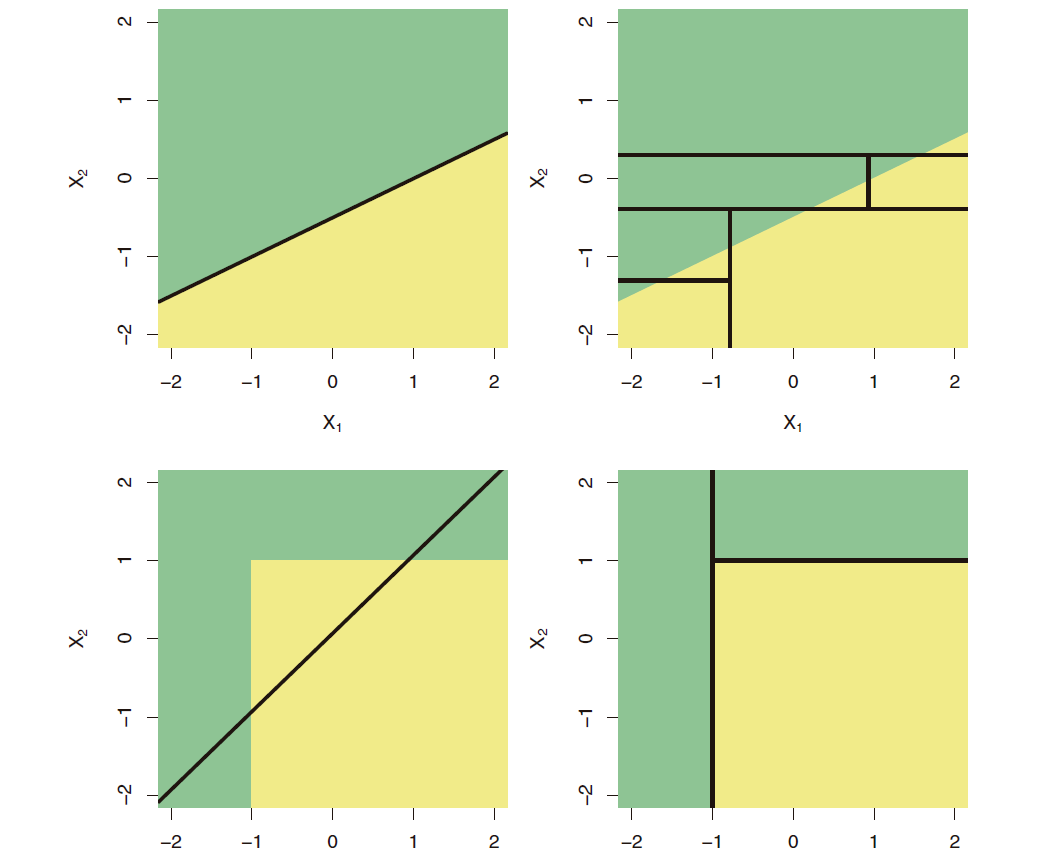
\includegraphics[scale=0.4]{svg-inkscape/compara.png}
\end{figure}
\end{frame}
\section{Mejoras}
\begin{frame}
\frametitle{Bagging}
\begin{enumerate}
	\item<1-> Coger muestras de las observaciones de entrenamiento.
	\item<2-> Formar para cada muestra un árbol.
	\item<3-> Si queremos hacer una predicción, hacemos 
	\begin{enumerate}
		\item La media de las predicciones de los árboles si es un modelo de regresión.
		\item La predicción mayoritaria si es un modelo de clasificación.
	\end{enumerate}
\end{enumerate}
\end{frame}

\begin{frame}
\frametitle{Random Forests}
Como bagging, pero cada árbol usa sólo algunos predictores.
\end{frame}

\begin{frame}
\frametitle{Boosting}
\begin{enumerate}
	\item<1-> Inicializar $r_i = y_i$.
	\item<2-> Para $b=1,2,\dots,B$:
	\begin{enumerate}
		\item Calcular un modelo de predicción basado en árbol $\widehat{f}^b$ para los datos $(X,r)$.
		\item Actualizar residuos:
		\[ r_i \leftarrow r_i - \lambda \widehat{f}^b(x_i) \]
	\end{enumerate}
	\item<3-> Devolver:
	\[ \widehat{f}(x) = \sum_{b=1}^B \lambda \widehat{f}^b(x) \]
\end{enumerate}
\end{frame}

\begin{frame}
\begin{figure}[h!]
\frametitle{Error respecto al parámetro de encogimiento}

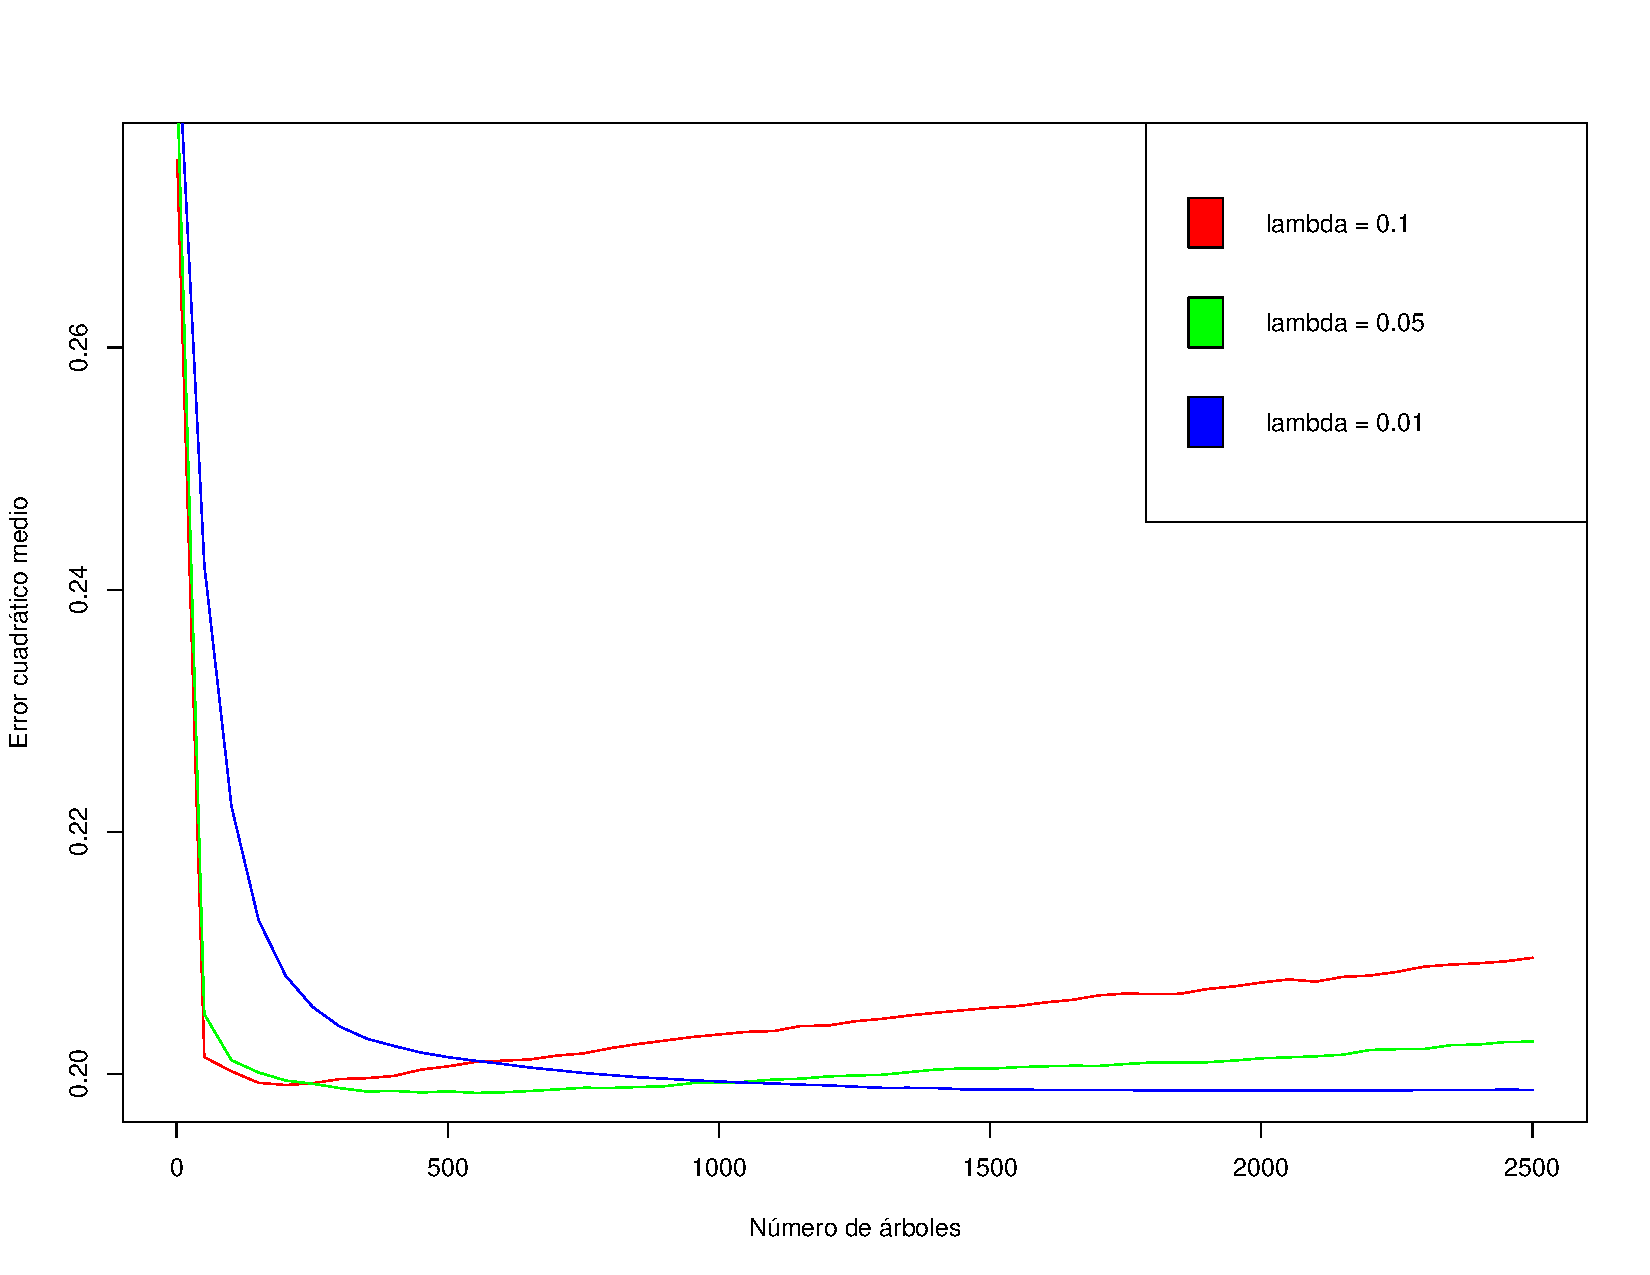
\includegraphics[scale=0.28]{shrinking}
\end{figure}
\end{frame}

\setbeamertemplate{headline}{}

\begin{frame}
\begin{figure}[h!]
Muchas gracias
\end{figure}
\end{frame}
\end{document}